\begin{figure}[htbp]
\centering
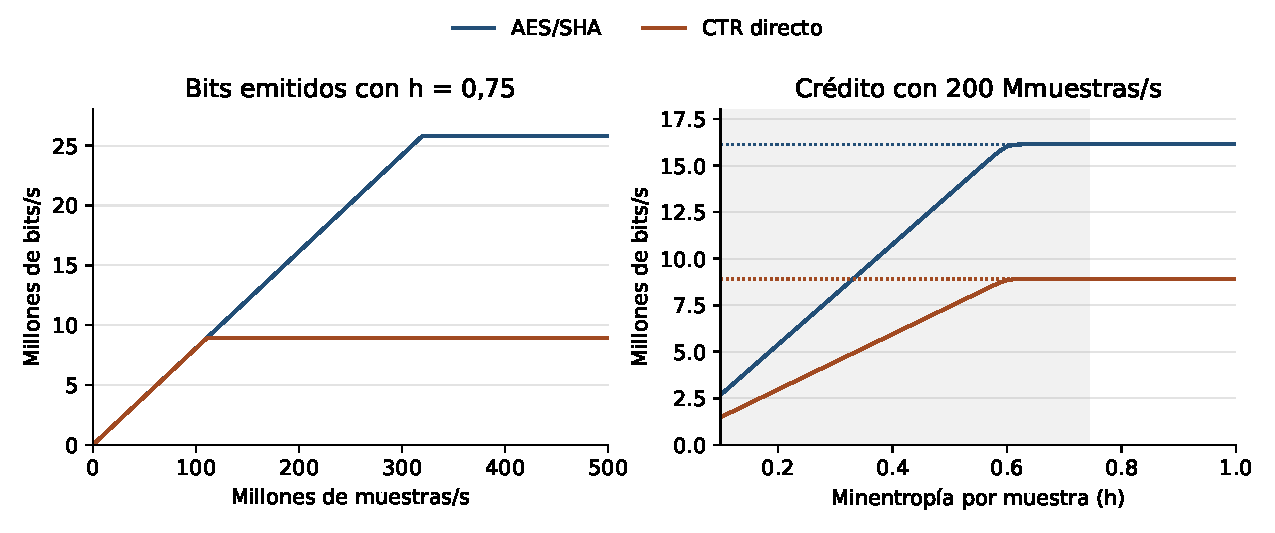
\includegraphics[width=\linewidth]{figures/port-rates.pdf}
\caption{Sensibilidad de los dos puertos directos. A la izquierda se varía la
frecuencia manteniendo \(h=0.75\) bits de minentropía por muestra. Las mesetas
proceden de los núcleos software medidos. A la derecha, para una adquisición
de 200 millones de muestras/s y una ventana fija de 427 muestras, las líneas
continuas dan la cota de minentropía condicional por segundo y las punteadas el
caudal de bits que admite la tubería. En la zona gris, las premisas numéricas
no acreditan el objetivo de distancia \(2^{-64}\) en \(2^{32}\) salidas mediante
la cota de extracción empleada: para ofertar ese servicio hay que redimensionar
la ventana o inhibir la entrega. Se usa el modelo clásico puntual, una muestra
binaria, aceptación de 0.99, dos incrementos por selector, guarda de 32 muestras,
\(\eta=2^{-160}\), épocas de 1024 llamadas y etapas solapadas. Los materiales
de semilla y su calidad se acreditan aparte.}
\label{fig:rate-sensitivity}
\end{figure}
